\documentclass{standalone}
\usepackage{tikz}
\usepackage{standalone}
\begin{document}
	
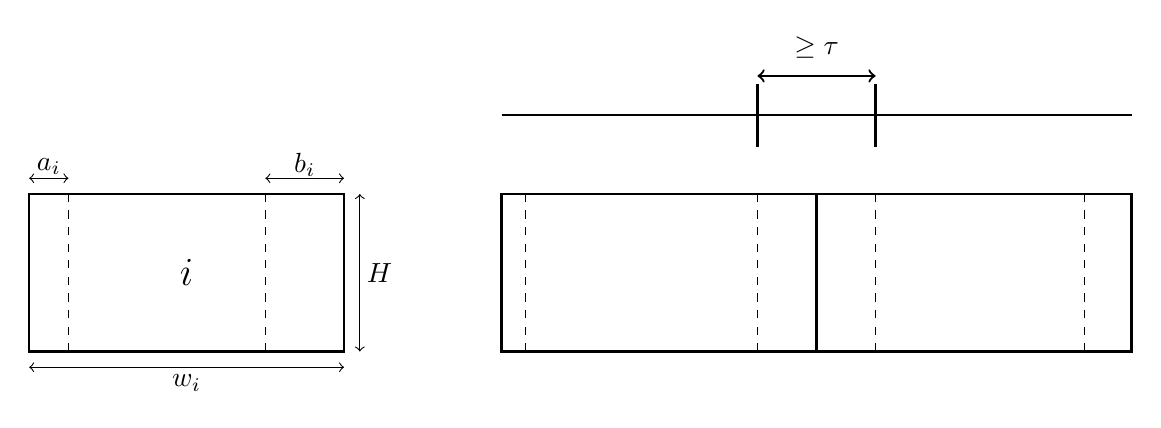
\begin{tikzpicture}
%\draw [help lines] (-7,-2) grid (9,5);

%\node at (-6.45, 1) {(a)};
%\node at (-0.45, 1) {(b)};

\draw [thick] (-6,0) rectangle (-2,2);
\draw [dashed] (-5.5,0) -- (-5.5, 2);
\draw [dashed] (-3.0,0) -- (-3.0, 2);

\draw [<->] (-6,-.2) -- (-2,-.2);
\node at (-4, -.4) {$w_i$};

\draw [<->] (-6, 2.2) -- (-5.5, 2.2);
\node at (-5.75, 2.35) {$a_i$};

\draw [<->] (-2, 2.2) -- (-3.0, 2.2);
\node at (-2.5, 2.375) {$b_i$};

\draw [<->] (-1.8,0) -- (-1.8,2);
\node at (-1.55,1) {$H$};

\node at (-4,1) {\Large{$i$}};


\draw [thick] (0,3) -- (8,3);
\draw [thick] (3.25,3.4) -- (3.25,2.6);
\draw [thick] (4.75,3.4) -- (4.75,2.6);
\draw [thick, <->] (3.25, 3.5) -- (4.75, 3.5);
\node [above] at (4,3.6) {$\geq \tau$};


\draw [thick] (0,0) rectangle (8,2);
\draw [thick] (4,2) -- (4,0);
\draw [dashed] (0.3,0) -- (0.3,2);
\draw [dashed] (3.25,0) -- (3.25,2);
\draw [dashed] (4.75,0) -- (4.75,2);
\draw [dashed] (7.4,0) -- (7.4,2);

%\draw [<->] (3.5,2.2) -- (4.5,2.2);
%\node at (4, -.4) {\scriptsize $\geq \tau$};







\end{tikzpicture}
	
\end{document}